\documentclass[11pt,letterpaper]{article}

% Load some basic packages that are useful to have
% and that should be part of any LaTeX installation.
%
% be able to include figures
\usepackage{graphicx}
% get nice colors
\usepackage{xcolor}

% change default font to Palatino (looks nicer!)
\usepackage{apjfonts}
% load some useful math symbols/fonts
\usepackage{latexsym,amsfonts,amsmath,amssymb}

% comfort package to easily set margins
\usepackage[top=1in, bottom=1in, left=1in, right=1in]{geometry}

% control some spacings
%
% spacing after a paragraph
\setlength{\parskip}{.15cm}
% indentation at the top of a new paragraph
\setlength{\parindent}{0.0cm}


\begin{document}

\begin{center}
\Large
{\bf Ay190 -- Worksheet 5} \\
\large
Xiangcheng Ma \\
Date: \today
\end{center}

\section*{Linear Fitting}
For convenience, I plot all the data and curves on a single plot.

(a) See the data point on Figure~\ref{fig}.

(b) The dashed line on Figure~\ref{fig} shows the linear fitting without consideration of uncertainty of measurement. The result is $\log(M_{\rm BH})=0.931+2.925\log(\sigma_*)$, in which $M_{\rm BH}$ is in unit of $M_{\odot}$ and $\sigma_*$ in $\rm km~s^{-1}$. While in Greene \& Ho (2006), their best fitting is 
$\log(M_{\rm BH})=-0.64+3.69\log(\sigma_*)$ (Dash-dot line in Figure~\ref{fig}). The difference is not significant.

(c) See the solid line in Figure~\ref{fig}. The result is $\log(M_{\rm BH})=0.342+3.232\log(\sigma_*)$

\begin{figure}[h]
\centering
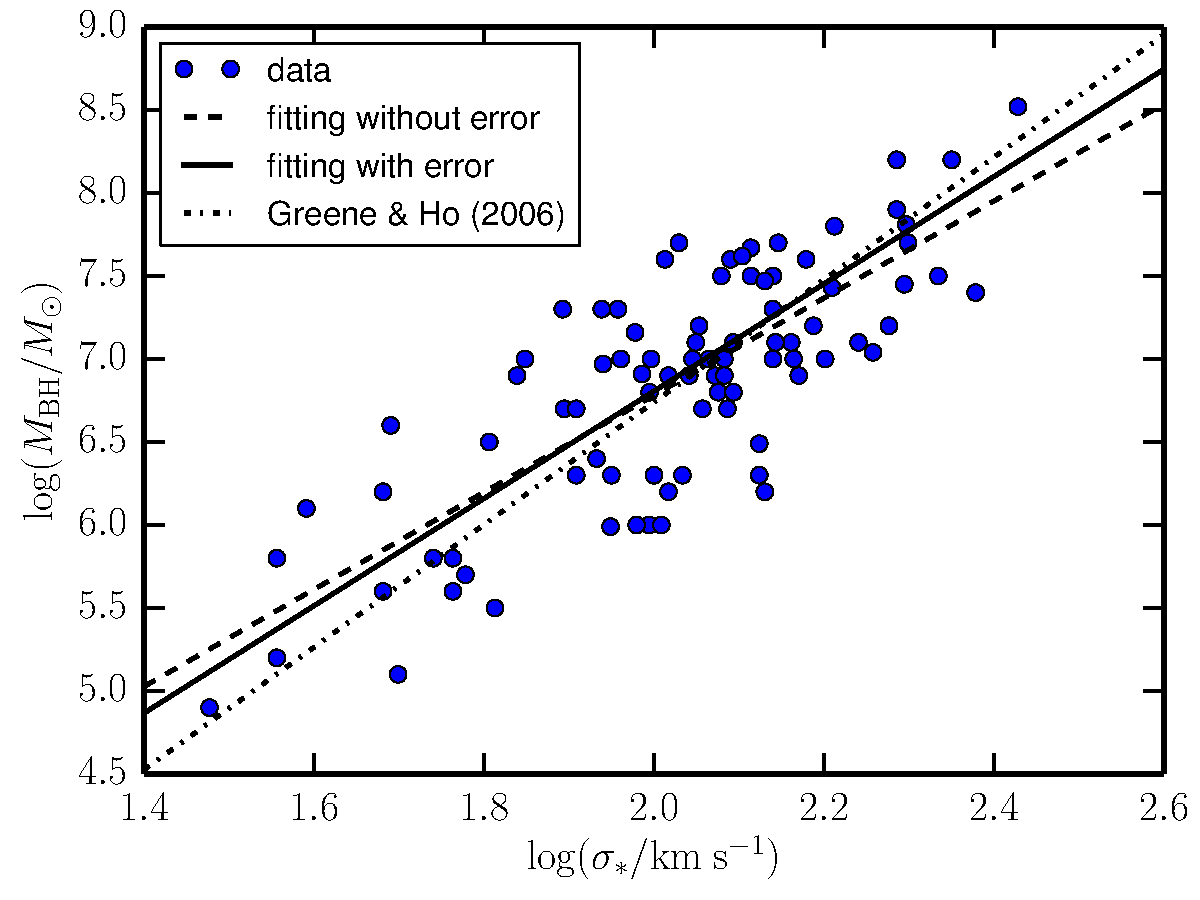
\includegraphics[width={0.99\textwidth}]{fig.pdf}
\caption{Linear Fitting}
\label{fig}
\end{figure}

\end{document}
